\documentclass{standalone}
\usepackage{amsmath}
\usepackage[T1]{fontenc}
\usepackage[utf8]{inputenc}

\usepackage[usenames,dvipsnames]{xcolor}

\usepackage{tikz}
\usetikzlibrary{arrows, shapes, matrix}

\begin{document}

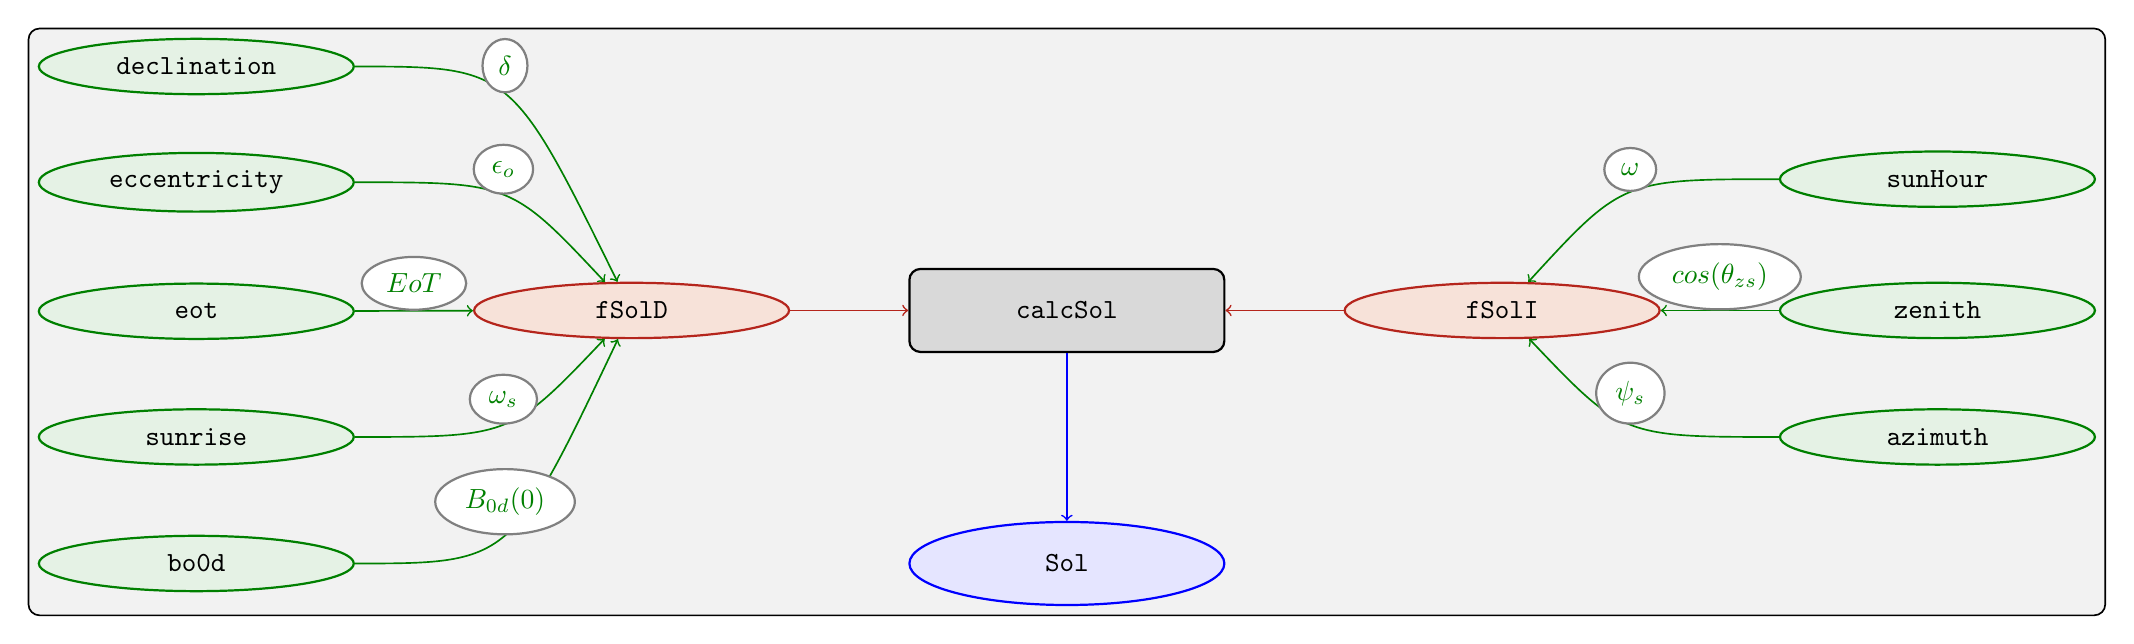
\begin{tikzpicture}[auto,
  method/.style={rectangle, rounded corners, draw=black, thick, fill=gray!30,
    minimum height = 3em, align=flush center, inner sep=1pt},
  %
  function/.style ={draw=BrickRed, thick, ellipse, fill=BrickRed!10,
    minimum height=2em},
  % 
  class/.style ={draw=Blue, thick, ellipse, fill=Blue!10,
    minimum height=3em},
  %
  utils/.style ={draw=Green, thick, ellipse, fill=Green!10,
    minimum height=2em},
  %
  simple/.style ={draw=black!50, thick, ellipse, fill=white}
  ]
  
  \tikzset{every path/.style={line width=.6pt}}

  \begin{scope}
    \matrix [matrix of nodes, rounded corners, fill=gray!10, draw=black, column
  sep=15mm,row sep=7mm, minimum width=4cm] (Geometry) {
    %%%%%%%%%%%%%%%%%%%%%%%%%%%%%%%
    \node [utils] (decl) {\texttt{declination}}; &
    \node {}; &
    \node {}; &
    \node {}; &
    \node {}; \\
    %%%%%%%%%%%%%%%%%%%%%%%%%%%%%%% 
    \node [utils] (eo) {\texttt{eccentricity}}; &
    \node {}; &
    \node {}; &
    \node {}; &
    \node [utils] (w) {\texttt{sunHour}}; \\
    %%%%%%%%%%%%%%%%%%%%%%%%%%%%%%%
    \node [utils] (EoT) {\texttt{eot}}; &
    \node [function] (fSolD) {\texttt{fSolD}}; &
    \node [method] (calcSol) {\texttt{calcSol}}; &
    \node [function] (fSolI) {\texttt{fSolI}}; &
    \node [utils] (cosThzS) {\texttt{zenith}}; \\
    %%%%%%%%%%%%%%%%%%%%%%%%%%%%%%%
    \node [utils] (ws) {\texttt{sunrise}}; &
    \node {}; &
    \node {}; &
    \node {}; &
    \node [utils] (AzS) {\texttt{azimuth}}; \\
    %%%%%%%%%%%%%%%%%%%%%%%%%%%%%%%
    \node [utils] (Bo0d) {\texttt{bo0d}}; &
    \node {}; &
    \node [class] (Sol) {\texttt{Sol}}; &
    \node {}; &
    \node {}; \\
  };
\end{scope}

\begin{scope}
  \draw [->, BrickRed] (fSolD) -- (calcSol);
  \draw [->, BrickRed] (fSolI) -- (calcSol);
  \draw [->, Blue] (calcSol) -- (Sol);
  \draw [->, Green] (decl) .. controls ++(0:4) .. (fSolD)
  node [midway, above, simple] {$\delta$};
  \draw [->, Green] (eo) .. controls ++(0:4) .. (fSolD)
  node [midway, above, simple] {$\epsilon_o$};
  \draw [->, Green] (EoT) -- (fSolD)
  node [midway, above, simple] {$EoT$};
  \draw [->, Green] (ws) .. controls ++(0:4) .. (fSolD)
  node [midway, above, simple] {$\omega_s$};
  \draw [->, Green] (Bo0d) .. controls ++(0:4) .. (fSolD)
  node [midway, above, simple] {$B_{0d}(0)$};
  \draw [->, Green] (w) .. controls ++(0:-4) .. (fSolI)
  node [midway, above, simple] {$\omega$};
  \draw [->, Green] (cosThzS) -- (fSolI)
  node [midway, above, simple] {$cos(\theta_{zs})$};
  \draw [->, Green] (AzS) .. controls ++(0:-4) .. (fSolI)
  node [midway, above, simple] {$\psi_s$};
  
\end{scope}
  
\end{tikzpicture}

\end{document}
